\chapter{Kísérletek, eredmények} 
\label{ch:results}

Ebben a fejezetben a releváns mérőszámok ismertetése után kiértékelem kísérletem eredményeit. Összevetem a kiinduló modell és saját fejlesztéseim teljesítményét a különböző bemeneti reprezentációkon.

\section{Mérőszámok}

A modellek teljesítményét F értékek alapján vetettem össze, egyrészt hangszerenként külön-külön, másrészt a hangszerenkénti átlagot véve is. Az F értékhez a következő metrikák vezettek el:

\begin{itemize}
\item \textbf{Pontosság (Accuracy)} - a modell helyes előrejelzéseinek száma osztva az összes előrejelzés számával. Ez már magában egy jó mérőszám tud lenni, azonban multi-label osztályozások esetén érdemes a helytelen előrejelzések fajtájával is kalkulálni. Ezek a valótlan igazak (false positives) és valótlan hamisak (false negatives).
\begin{figure}[H]
  \centering
  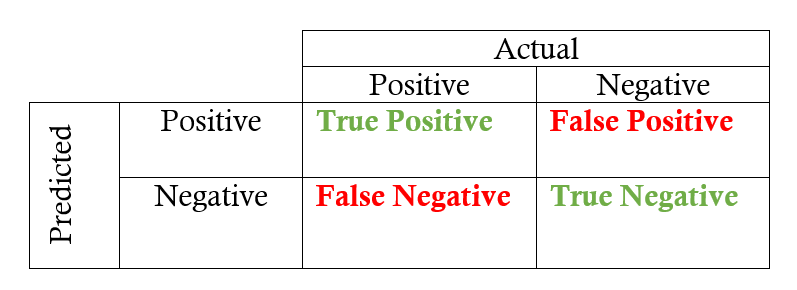
\includegraphics[width=\textwidth]{predictedactual.png}
  \caption{Előrejelzések fajtái, forrás: \cite{fscore}}
\end{figure}

\item \textbf{Hiba (Loss)} - a hibafüggvény eredménye. A modell predikcióinak a valóságtól való eltérését összeadva kapjuk meg. A modell célja tanuláskor ennek az értéknek a minimalizálása.
\item \textbf{Precizitás (Precision)} - valós igaz predikációk száma osztva a valós és valótlan igaz predikációk számának összegével.
\item \textbf{Felidézés (Recall)} - valós igaz predikációk száma osztva a valós igaz és valótlan hamis predikációk összegével.
\begin{figure}[H]
  \centering
  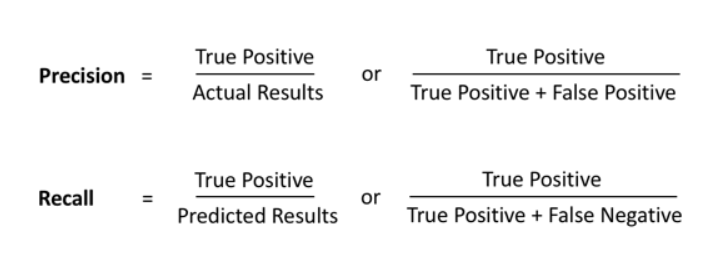
\includegraphics[width=\textwidth]{precisionrecall.png}
  \caption{Precizitás és felidézés, forrás: \cite{fscore}}
\end{figure}
\item \textbf{F érték (F score)} - a precizitás és felidézés értékek harmonikus közepe. Ez lesz tehát a meghatározó mérőszám a modelljeink összevetésénél. \cite{fscore}

\begin{figure}[H]
  \centering
  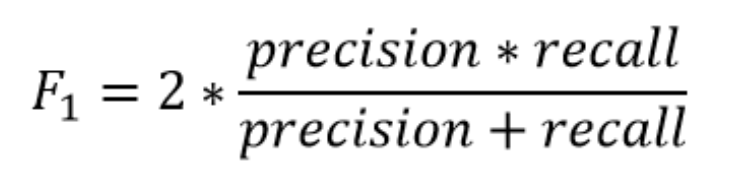
\includegraphics[width=6cm]{fscore.png}
  \caption{F score képlete, forrás: \cite{fscore}}
\end{figure}
\end{itemize}



\section{Eredmények}

A végső eredmények csak az OpenMIC datasettel kapcsolatos kísérleteket tartalmazzák. Az eredmények összevetésére a hangszerenkénti F értékeket használtam fel. Ez modellenként 20 hangszer, ami 20 különböző értéket jelent. Ezért minden modell végső összevetési alapjának két összesítő értéket választottam: az F értékek átlagát és a 0,70 feletti F értéket meghaladó hangszerek számát. Utóbbira a továbbiakban jól tanított hangszerként fogok hivatkozni. Saját intuícióm vezetett arra a következtetésre, hogy 0,70-es F érték felett már életszerűen használható értékről beszélhetünk.

A továbbiakban a Modeling Baseline és a Shallow CNN architektúrák különböző eredményeit mutatom be. Az eredményeket mindenhol többszöri futtatás maximálisan elért értékei reprezentálják.

\subsection{VGGish kiindulás}

Először a VGGish reprezentáció tekintetében tettem kísérleteket, mivel a Modeling Baseline eredeti implementációja ezt használta fel. Első lépésként ezt futtattam módosítás nélkül, majd lecseréltem a felhasznált RFC-t a saját CNN architektúrámra.

\begin{figure}[H]
\centering
\begin{tikzpicture}
    \begin{axis}[
        width  = \textwidth,
        height = 7cm,
        major x tick style = transparent,
        ybar=0pt,
        bar width=4pt,
        ymajorgrids = true,
        ylabel = {F érték},
        symbolic x coords={Harmónika,Bendzsó,Basszusgitár,Cselló,Klarinét,Cintányér,Dob,Furulya,Gitár,Melodikus ütőhangszer,Mandolin,Orgona,Zongora,Szaxofon,Szintetizátor,Harsona,Trombita,Ukulele,Hegedű,Ének},
        xtick = data,
        x tick label style={rotate=90},
        scaled y ticks = false,
        legend cell align=left,legend style={
                at={(1,1.05)},
                anchor=south east,
                column sep=1ex}
    ]
        \addplot[style={bblue,fill=bblue,mark=none}]
            coordinates {(Harmónika, 0.68) (Bendzsó,0.72) (Basszusgitár,0.75)  (Cselló,0.79)  (Klarinét,0.52)  (Cintányér,0.93)  (Dob,0.75)  (Furulya,0.89)  (Gitár,0.97)  (Melodikus ütőhangszer,0.77)  (Mandolin,0.70)  (Orgona,0.60) (Zongora,0.93) (Szaxofon,0.83) (Szintetizátor,0.94) (Harsona,0.75) (Trombita,0.76) (Ukulele,0.72) (Hegedű,0.83) (Ének,0.93)};
        \addplot[style={rred,fill=rred,mark=none}]
            coordinates {(Harmónika, 0.76) (Bendzsó,0.74) (Basszusgitár,0.66) (Cselló,0.73) (Klarinét,0.52)  (Cintányér,0.88) (Dob,0.93) (Furulya,0.66) (Gitár,0.95)  (Melodikus ütőhangszer,0.79)  (Mandolin,0.64)  (Orgona,0.77) (Zongora,0.91) (Szaxofon,0.67) (Szintetizátor,0.89) (Harsona,0.77) (Trombita,0.71) (Ukulele,0.64) (Hegedű,0.76) (Ének,0.81)};
        \legend{Modeling Baseline, Shallow CNN}
    \end{axis}
\end{tikzpicture}
\caption{Modeling Baseline és Shallow CNN eredményei optimalizációk nélkül VGGish reprezentáción} \label{fig:vggishbase}
\end{figure}

Az eredmények hangszerenként a \ref{fig:vggishbase} ábrán láthatóak. Az F értékek átlaga és a jól tanított hangszerek száma kicsivel magasabb volt a Modeling Baseline modellen, mint a Shallow CNN-en. Előbbi 0,79 átlag F értéket és 17 jól tanított hangszert, utóbbi 0,76 átlag F értéket és 14 jól tanított hangszert produkált.

Ami még leolvasható a \ref{fig:vggishbase} ábráról, hogy a hangszerek között vannak jobban és kevésbé taníthatóak. Például a klarinét és a mandolin mindkét modellen relatív alacsony F értéket hozott. Ezzel szemben a gitár és a zongora tanítása mindkét modell esetében 0.9 feletti F értéket eredményezett.

A hangszereket vizsgálva a modellek között megjelentek nagyon hasonló és különböző értékek is. A legnagyobb különbséget a Shallow CNN javára a dob mutatta, itt 0,75 állt szemben 0,93-mal, ami 0,18 F érték eltérés. A Modeling Baseline javára pedig a furulyával kapcsolatos számok jelentették a legnagyobb, 0,23 F értéknyi eltérést. Itt 0,66 és 0,89 volt a két érték.

\subsection{Optimalizáció}

Következő lépésként implementáltam a különböző előfeldolgozási adatoptimalizáló technikákat, mint például undersampling és normalizáció. Ezután szintén a VGGish reprezentáción futtatva a modellek teljesítménye javulást ért el: mindkét modell F érték átlaga egyaránt 0,83-ra növekedett a korábbi 0,79-ről és 0,76-ról. Ezenfelül a jól tanított hangszerek száma mindkét modell esetén elérte a maximális 20-at a korábbi 17 és 14 helyett. Ez a ShallowCNN számára magasabb relatív javulást jelent, ennek hangszerenkénti összevetése a \ref{fig:shallowcnnopt} ábrán látható.

\begin{figure}[H]
\centering
\begin{tikzpicture}
    \begin{axis}[
        width  = \textwidth,
        height = 7cm,
        major x tick style = transparent,
        ybar=0pt,
        bar width=4pt,
        ymajorgrids = true,
        ylabel = {F érték},
        symbolic x coords={Harmónika,Bendzsó,Basszusgitár,Cselló,Klarinét,Cintányér,Dob,Furulya,Gitár,Melodikus ütőhangszer,Mandolin,Orgona,Zongora,Szaxofon,Szintetizátor,Harsona,Trombita,Ukulele,Hegedű,Ének},
        xtick = data,
        x tick label style={rotate=90},
        scaled y ticks = false,
        legend cell align=left,legend style={
                at={(1,1.05)},
                anchor=south east,
                column sep=1ex}
    ] 
        \addplot[style={rred,fill=rred,mark=none}]
            coordinates {(Harmónika, 0.76) (Bendzsó,0.74) (Basszusgitár,0.66) (Cselló,0.73) (Klarinét,0.52)  (Cintányér,0.88) (Dob,0.93) (Furulya,0.66) (Gitár,0.95)  (Melodikus ütőhangszer,0.79)  (Mandolin,0.64)  (Orgona,0.77) (Zongora,0.91) (Szaxofon,0.67) (Szintetizátor,0.89) (Harsona,0.77) (Trombita,0.71) (Ukulele,0.64) (Hegedű,0.76) (Ének,0.81)};
       \addplot[style={ggreen,fill=ggreen,mark=none}]
            coordinates {(Harmónika, 0.74) (Bendzsó,0.81) (Basszusgitár,0.75) (Cselló,0.77) (Klarinét,0.72)  (Cintányér,0.93) (Dob,0.93) (Furulya,0.72) (Gitár,0.96)  (Melodikus ütőhangszer,0.79)  (Mandolin,0.79)  (Orgona,0.82) (Zongora,0.96) (Szaxofon,0.8) (Szintetizátor,0.96) (Harsona,0.81) (Trombita,0.81) (Ukulele,0.74) (Hegedű,0.84) (Ének,0.96)};
        \legend{Kezdeti,Optimalizált}
    \end{axis}
\end{tikzpicture}
\caption{Shallow CNN eredményei VGGish reprezentáción optimalizációk előtt, illetve után}
\label{fig:shallowcnnopt}
\end{figure}

Így végül az optimalizált adathalmazon -, bár hangszerenként vannak kisebb eltérések mindkét megoldás irányába - összesítve ugyanolyan eredményt képes produkálni egy hagyományos gépi tanulási algoritmus, mint egy mély tanulási modell. Legalábbis a kis méretű, előre tanított VGGish reprezentáción.

\subsection{Alternatív reprezentációk}

A VGGish reprezentáció után mindkét modellt futtattam melspectogram és MFCC reprezentációkat felhasználva. A melspectogram tekintetében végeztem az adatoptimalizálás előtt is kísérleteket. Már itt is észrevehető volt, hogy a mély tanulás a nagyobb, komplexebb reprezentáción jobb eredményt mutat. A Modeling Baseline 0,56-os átlag F értéket és négy jól tanított hangszert, a Shallow CNN architektúra pedig 0,61-es átlag F értéket és öt jól tanított hangszert produkált.

Ám az adatoptimalizáció utáni értékek még jelentősebbek. Az optimalizáció kapcsán lényegében ugyanaz látszik, mint a VGGish esetén: mindkét modellen javulást eredményezett az optimalizálás, de a Shallow CNN-en szignifikánsabb a különbség. A végső értékek a Modeling Baseline tekintetében 0,65-ös átlag F érték és öt jól tanított hangszer. Ezzel szemben a Shallow CNN átlag F értéke 0,73-ra, jól tanított hangszereinek száma 12-re nőtt. Ez a Modeling Baseline esetén plusz 0,09 átlag F értéket és egy jól tanított hangszert jelent, míg a Shallow CNN esetén plusz 0,12 átlag F értéket és hét jól tanított hangszert. Így tehát a Modeling Baseline és Shallow CNN melspectogramon vett végső eredményei közül a Shallow CNN-é magasabb 0,08 átlag F értékkel és hét jól tanított hangszerrel. A hangszerenkénti értékek a \ref{fig:melspec} ábráról olvashatóak le.

\begin{figure}[H]
\centering
\begin{tikzpicture}
    \begin{axis}[
        width  = \textwidth,
        height = 7cm,
        major x tick style = transparent,
        ybar=0pt,
        bar width=4pt,
        ymajorgrids = true,
        ylabel = {macro f-score},
        symbolic x coords={Harmónika,Bendzsó,Basszusgitár,Cselló,Klarinét,Cintányér,Dob,Furulya,Gitár,Melodikus ütőhangszer,Mandolin,Orgona,Zongora,Szaxofon,Szintetizátor,Harsona,Trombita,Ukulele,Hegedű,Ének},
        xtick = data,
        x tick label style={rotate=90},
        scaled y ticks = false,
legend cell align=left,legend style={
                at={(1,1.05)},
                anchor=south east,
                column sep=1ex
        }
    ]
        \addplot[style={ppurple,fill=ppurple,mark=none}]
            coordinates {(Harmónika,0.65) (Bendzsó,0.55) (Basszusgitár,0.63) (Cselló,0.64)  (Klarinét,0.63)  (Cintányér,0.79)  (Dob,0.83)  (Furulya, 0.60)  (Gitár,0.59)  (Melodikus ütőhangszer,0.60)  (Mandolin,0.55)  (Orgona,0.73) (Zongora,0.91) (Szaxofon,0.56) (Szintetizátor,0.58) (Harsona,0.62) (Trombita,0.64) (Ukulele,0.57) (Hegedű,0.61) (Ének,0.81) };

        \addplot[style={oorange,fill=oorange,mark=none}]
            coordinates {(Harmónika,0.69) (Bendzsó,0.64) (Basszusgitár,0.72) (Cselló,0.71)  (Klarinét,0.61)  (Cintányér,0.86)  (Dob,0.90)  (Furulya,0.64)  (Gitár,0.84)  (Melodikus ütőhangszer,0.46)  (Mandolin,0.69)  (Orgona,0.76) (Zongora,0.91) (Szaxofon,0.68) (Szintetizátor,0.81) (Harsona,0.72) (Trombita,0.75) (Ukulele,0.64) (Hegedű,0.76) (Ének,0.81) };
 	
 	
        \legend{Modeling Baseline, Shallow CNN}
    \end{axis}
\end{tikzpicture}
\caption{Modeling Baseline és Shallow CNN eredményei melspectogram reprezentáción adatoptimalizáció után}
\label{fig:melspec}
\end{figure}

A melspectogram reprezentáció után az MFCC következett. Az MFCC reprezentáción mindkét modell a melspectogramon való futtatáshoz hasonló eredményt adott. A Modeling Baseline 0,61-es átlag F értéket és négy jól tanított hangszert ért el, ez 0,04 átlag F értékkel és egy jól tanított hangszerrel alacsonyabb, mint melspectogram esetén. A Shallow CNN tekintetében pedig 0,72 átlag F érték és nyolc jól tanított hangszer lett a végső eredmény. Ezek az értékek 0,01 átlag F érték és négy jól tanított hangszernyi különbséget mutatnak a melspectogram javára. A hangszerenkénti értékek a \ref{fig:mfcc} ábráról olvashatóak le.

\begin{figure}[H]
\centering
\begin{tikzpicture}
    \begin{axis}[
        width  = \textwidth,
        height = 7cm,
        major x tick style = transparent,
        ybar=0pt,
        bar width=4pt,
        ymajorgrids = true,
        ylabel = {F érték},
        symbolic x coords={Harmónika,Bendzsó,Basszusgitár,Cselló,Klarinét,Cintányér,Dob,Furulya,Gitár,Melodikus ütőhangszer,Mandolin,Orgona,Zongora,Szaxofon,Szintetizátor,Harsona,Trombita,Ukulele,Hegedű,Ének},
        xtick = data,
        x tick label style={rotate=90},
        scaled y ticks = false,
legend cell align=left,legend style={
                at={(1,1.05)},
                anchor=south east,
                column sep=1ex
        }
    ]
        \addplot[style={oorange,fill=oorange,mark=none}]
            coordinates {(Harmónika,0.69) (Bendzsó,0.64) (Basszusgitár,0.72) (Cselló,0.71)  (Klarinét,0.61)  (Cintányér,0.86)  (Dob,0.90)  (Furulya,0.64)  (Gitár,0.84)  (Melodikus ütőhangszer,0.46)  (Mandolin,0.69)  (Orgona,0.76) (Zongora,0.91) (Szaxofon,0.68) (Szintetizátor,0.81) (Harsona,0.72) (Trombita,0.75) (Ukulele,0.64) (Hegedű,0.76) (Ének,0.81) };
            
        \addplot[style={bbrown,fill=bbrown,mark=none}]
            coordinates {(Harmónika,0.66) (Bendzsó,0.61) (Basszusgitár,0.71) (Cselló,0.71)  (Klarinét,0.66)  (Cintányér,0.87)  (Dob,0.83)  (Furulya, 0.66)  (Gitár,0.88)  (Melodikus ütőhangszer,0.60)  (Mandolin,0.63)  (Orgona,0.71) (Zongora,0.93) (Szaxofon,0.65) (Szintetizátor,0.81) (Harsona,0.67) (Trombita,0.68) (Ukulele,0.62) (Hegedű,0.79) (Ének,0.81) };
 	
 	
        \legend{melspectogram, MFCC}
    \end{axis}
\end{tikzpicture}
\caption{Shallow CNN végső eredményei melspectogram és MFCC reprezentáción}
\label{fig:mfcc}
\end{figure}

Melspectogram, illetve MFCC reprezentációk közti jelentős hatékonyságbeli különbség tehát nem jelenik meg az eredményekben. Ezt érdemes lenne tovább vizsgálni. Az különbségek bizonyításához vagy cáfolásához mélyebb architektúrára, valamint több bemeneti adatra lenne szükség.

\subsection{Összehasonlítás}

A bemutatott eredményekből és a \ref{tab:all} összefoglaló táblázatból látszik, hogy melspectogram és MFCC bemeneti reprezentációk esetén az általam prezentált deep learning architektúra (Shallow CNN) jobb eredményeket produkál, mint egy hagyományos gépi tanulási algoritmus (Modeling Baseline).

\begin{table}[H]
	\centering
	\begin{tabular}{ | c | p{2,5cm} | p{2,5cm} |}
		\hline
		 & \textbf{Átlagos F érték} & \textbf{Jól tanított hangszerek száma}  \\
		\hline \hline
		\emph{Modeling Baseline VGGish kezdeti} & 0,79 & 17 \\
		\hline
		\emph{Shallow CNN VGGish kezdeti} & 0,76 & 14  \\
		\hline
		\emph{Modeling Baseline melspectogram kezdeti} & 0,56 & 4 \\
		\hline
		\emph{Shallow CNN melspectogram kezdeti} & 0,61 & 5 \\
		\hline
		\emph{Modeling Baseline MFCC kezdeti} & Nincs adat & Nincs adat \\
		\hline
		\emph{Shallow CNN MFCC kezdeti} & Nincs adat & Nincs adat \\
		\hline
		\emph{Modeling Baseline VGGish optimalizált} & 0,83 & 20\\
		\hline
		\emph{Shallow CNN VGGish optimalizált} & 0,83 & 20 \\
		\hline
		\emph{Modeling Baseline melspectogram optimalizált} & 0,65 & 5 \\
		\hline
		\emph{Shallow CNN melspectogram optimalizált} & 0,73 & 12 \\
		\hline
		\emph{Modeling Baseline MFCC optimalizált} & 0,61 & 4 \\
		\hline
		\emph{Shallow CNN MFCC optimalizált} & 0,72 & 8 \\
		\hline
	\end{tabular}
	\caption{Kísérletek és eredmények összefoglalva}
	\label{tab:all}
\end{table}


A reprezentációk tekintetében elmondható, hogy a melspectogram és MFCC jelentősen gyengébb eredményeket értek el, mint a VGGish. Ennek fő oka az adathalmaz méretéből fakad, ugyanis a VGGish reprezentációt célzottan  sekélyebb architektúrákra, kevesebb adatra alkották meg.